\documentclass[a4paper,oneside]{report}

\usepackage[utf8]{inputenc}
\usepackage{polski}
\usepackage{color}
\usepackage{listings}
\usepackage[pdftex]{graphicx}
\usepackage{tikz}
\usetikzlibrary{matrix,calc}
\usepackage{amsmath}

\newcommand{\startstop}{\texttt{START/STOP}}
\newcommand{\reset}{\texttt{RESET}}
\newcommand{\addmin}{\texttt{ADD\textunderscore MIN}}
\newcommand{\addsec}{\texttt{ADD\textunderscore SEC}}
\newcommand{\clocksec}{\texttt{clock\textunderscore sec}}
\newcommand{\debouncer}{\texttt{debouncer}}
\newcommand{\counter}[1]{\texttt{counter\textunderscore #1}}
\newcommand{\mode}{\texttt{mode}}
\newcommand{\bcdtoseg}{\texttt{bcd\textunderscore to\textunderscore 7seg}}
\newcommand{\tff}{\texttt{t\textunderscore ff}}

%% Karnaugh
\def\n#1{\overline{#1}}
\def\s#1{\scriptsize #1}
%Empty Karnaugh map 4x4
\newenvironment{Karnaugh}{
\begin{tikzpicture}[baseline=(current bounding box.north),scale=0.8]
\draw (0,0) grid (4,4);
%
\matrix (mapa) [matrix of nodes,
        column sep={0.8cm,between origins},
        row sep={0.8cm,between origins},
        every node/.style={minimum size=0.3mm},
        anchor=2.center,
        ampersand replacement=\&] at (0.5,0.5)
{
|(name)| \phantom{F}   \& 
|(c00)| \s$\n{Q_3Q_2}$  \& 
|(c01)| \s$\n{Q_3}Q_2$  \& 
|(c11)| \s$Q_3Q_2$      \& 
|(c10)| \s$Q_3\n{Q_2}$  \& 
|(cf)| \phantom{00} \\
%
|(r00)| \s$\n{Q_1Q_0}$ \& |(0)|  \phantom{0} \& |(4)|  \phantom{0} \& |(12)| \phantom{0} \& |(8)|  \phantom{0} \& \\
|(r01)| \s$\n{Q_1}Q_0$ \& |(1)|  \phantom{0} \& |(5)|  \phantom{0} \& |(13)| \phantom{0} \& |(9)|  \phantom{0} \& \\
|(r11)| \s$Q_1Q_0$     \& |(3)|  \phantom{0} \& |(7)|  \phantom{0} \& |(15)| \phantom{0} \& |(11)| \phantom{0} \& \\
|(r10)| \s$Q_1\n{Q_0}$ \& |(2)|  \phantom{0} \& |(6)|  \phantom{0} \& |(14)| \phantom{0} \& |(10)| \phantom{0} \& \\
|(rf) | \phantom{00}   \&                    \&                    \&                    \&                    \& \\
};
}{\end{tikzpicture}}

\newcommand{\contingut}[1]{% fill values
  \foreach \x [count=\xi from 0] in {#1} 
    \path (\xi) node {\x};
}
% Grouping on Karnaugh maps
\newcommand{\grpone}[3][0]{ % group one [padding] {node} {color}
\draw[rounded corners=3pt, fill=#3, opacity=0.3] ($(#2.north west)+(135:#1)$) rectangle ($(#2.south east)+(-45:#1)$);
}
\newcommand{\grp}[4][0]{ % group internal [padding] {top-left} {bottom-right} {color}
\draw[rounded corners=3pt, fill=#4, opacity=0.3] ($(#2.north west)+(135:#1)$) rectangle ($(#3.south east)+(-45:#1)$);
}
\newcommand{\grph}[4][0]{ % group lateral borders [padding] {top-left} {bottom-right} {color}
\draw[rounded corners=3pt, fill=#4, opacity=0.3] ($(rf.east |- #2.north)+(90:#1)$)-| ($(#2.east)+(0:#1)$) |- ($(rf.east |- #3.south)+(-90:#1)$);
\draw[rounded corners=3pt, fill=#4, opacity=0.3] ($(cf.west |- #2.north)+(90:#1)$) -| ($(#3.west)+(180:#1)$) |- ($(cf.west |- #3.south)+(-90:#1)$);
}
\newcommand{\grpv}[4][0]{ % group top-bottom borders [padding] {top-left} {bottom-right} {color}
\draw[rounded corners=3pt, fill=#4, opacity=0.3] ($(cf.south -| #2.west)+(180:#1)$) |- ($(#2.south)+(-90:#1)$) -| ($(cf.south -| #3.east)+(0:#1)$);
\draw[rounded corners=3pt, fill=#4, opacity=0.3] ($(rf.north -| #2.west)+(180:#1)$) |- ($(#3.north)+(90:#1)$) -| ($(rf.north -| #3.east)+(0:#1)$);
}
\newcommand{\grpc}[2][0]{ % group corners [padding] {color}
\draw[rounded corners=3pt, opacity=.3] ($(rf.east |- 0.south)+(-90:#1)$) -| ($(0.east |- cf.south)+(0:#1)$);
\draw[rounded corners=3pt, opacity=.3] ($(rf.east |- 2.north)+(90:#1)$) -| ($(2.east |- rf.north)+(0:#1)$);
\draw[rounded corners=3pt, opacity=.3] ($(cf.west |- 8.south)+(-90:#1)$) -| ($(8.west |- cf.south)+(180:#1)$);
\draw[rounded corners=3pt, opacity=.3] ($(cf.west |- 10.north)+(90:#1)$) -| ($(10.west |- rf.north)+(180:#1)$);
\fill[rounded corners=3pt, fill=#2, opacity=.3] ($(rf.east |- 0.south)+(-90:#1)$) -|  ($(0.east |- cf.south)+(0:#1)$) [sharp corners] ($(rf.east |- 0.south)+(-90:#1)$) |-  ($(0.east |- cf.south)+(0:#1)$) ;
\fill[rounded corners=3pt, fill=#2, opacity=.3] ($(rf.east |- 2.north)+(90:#1)$) -| ($(2.east |- rf.north)+(0:#1)$) [sharp corners] ($(rf.east |- 2.north)+(90:#1)$) |- ($(2.east |- rf.north)+(0:#1)$) ;
\fill[rounded corners=3pt, fill=#2, opacity=.3] ($(cf.west |- 8.south)+(-90:#1)$) -| ($(8.west |- cf.south)+(180:#1)$) [sharp corners]($(cf.west |- 8.south)+(-90:#1)$) |- ($(8.west |- cf.south)+(180:#1)$) ;
\fill[rounded corners=3pt, fill=#2, opacity=.3] ($(cf.west |- 10.north)+(90:#1)$) -| ($(10.west |- rf.north)+(180:#1)$) [sharp corners] ($(cf.west |- 10.north)+(90:#1)$) |- ($(10.west |- rf.north)+(180:#1)$) ;
}
% Karnaugh ends here

\definecolor{dkgreen}{rgb}{0,0.6,0}
\definecolor{gray}{rgb}{0.5,0.5,0.5}
\definecolor{mauve}{rgb}{0.58,0,0.82}

\lstset{frame=shadowbox,
  language=Verilog,
  aboveskip=3mm,
  belowskip=3mm,
  showstringspaces=false,
  columns=flexible,
  basicstyle={\small\ttfamily},
  numbers=none,
  numberstyle=\tiny\color{gray},
  keywordstyle=\color{blue},
  commentstyle=\color{dkgreen},
  stringstyle=\color{mauve},
  breaklines=true,
  breakatwhitespace=true,
  tabsize=3
}

%% START:

\title{
	\textbf{Technika cyfrowa}
	\\
	Timer (\texttt{MM:SS}) z ustawianiem czasu
	}
\author{
	Paweł Maniecki\\
	Filip Galas
	}
\date{Rok akademicki: 2014/2015}

\begin{document}
\maketitle

\tableofcontents
\listoffigures

\chapter{Instrukcja użytkownika}
\section{Opis działania.}
Celem projektu jest \emph{timer} zrealizowany na zestawie
edukacyjnym Altera UP2.

Timer wyposażony jest w licznik czasu (\texttt{MM:SS}), którego
stan widoczny jest na wyświetlaczu. Z punktu widzenia użytkownika
układ może znajdować się w jednym z dwóch trybów, pomiędzy którymi
można przestawiać się przyciskiem \startstop :
\begin{enumerate}
\item Tryb \emph{zliczania}.\\
W tym trybie licznik zlicza czas w dół. Działanie przycisków
\reset , \addmin\ i \addsec\ jest zablokowane.
\item Tryb \emph{ustawiania}.\\
W tym trybie zliczanie czasu jest zatrzymane. Możliwe jest
dodawanie minut i/lub sekund do licznika przyciskami \addmin\ i
\addsec\ oraz zresetowanie jego stanu przyciskiem \reset .
\end{enumerate}
Gdy licznik podczas zliczania osiągnie stan \texttt{00:00}, układ
zasygnalizuje to miganiem cyfr na wyświetlaczach LED. Po
wciśnięciu przycisku \startstop\ timer powróci do trybu
\emph{ustawiania}.
\section{Opis interfejsu użytkownika.}
Aktualny stan timera w fromacie \texttt{MM.SS} wyświetlany jest na czterech wyświetlaczach 
7-segmentowych znajdujących się na \emph{płytce rozszerzeń C}. 

Sterowanie układem odbywa się w całości przy pomocy przycisków chwilowych na \emph{płytce A}. 
Układ przycisków, ich oznaczenia na płytce i nazwy używane w instrukcji widoczne są poniżej:
\begin{table}[h] \centering
  \renewcommand{\arraystretch}{2}
  \begin{tabular}{r|c|c|l} \cline{2-3}
  \addmin & \texttt{BT3} & \texttt{BT2} & \addsec    \\ \cline{2-3}
  \reset  & \texttt{BT1} & \texttt{BT0} & \startstop \\ \cline{2-3}
  \end{tabular}
\end{table}

Funkcje przycisków:
\begin{itemize}
	\item \startstop\ --- zatrzymywanie/uruchamianie timera
	\item \addsec\ --- dodawanie sekund do licznika (tylko w trybie
		\emph{ustawiania})
	\item \addmin\ --- dodawanie minut do licznika (tylko w trybie
		\emph{ustawiania})
	\item \reset\ --- resetowanie timera (tylko w trybie
		\emph{ustawiania})
\end{itemize}

\chapter{Realizacja projektu}
\section{Układ timera.}
\subsection{Ogólny schemat.}
Układ timera oparty jest na czterech licznikach: dwóch licznikach
modulo 6 oraz dwóch --- modulo 10. Na rysunku \ref{timer_scheme}
przedstawiamy uproszczony schemat układu, który ułatwia zrozumienie
jego idei.

Każdy licznik odpowiada za jedną z cyfr wg schematu: \texttt{MM:SS}.
Cyfry jedności należą do przedziału [0..9], zaś cyfry dziesiątek ---
[0..5]. \emph{Przeniesienia} cyfr jedności połączone są z wejściami
cyfr dziesiątek odpowiadających za \emph{inkrementację}.
Analogicznie, \emph{pożyczki} połączone są z wejściami
\emph{dekrementacji}. Do wejść licznika sekundowych cyfr jedności
poprowadzone są sygnały odpowiednio: sygnał pochodzący z przycisku
\addsec\ do inkrementacji, sygnał zegara 1Hz, poprzez odpowiedni
przełącznik (szczegóły w dalszej części sprawozdania) --- do
dekrementacji. Do wejść licznika minutowych cyfr jedności
doprowadzone są sygnały: do wejścia inkrementacji --- sygnał z
przycisku \addmin , zaś do dekrementacji --- pożyczka z sekundowej
cyfry jedności. Oprócz tego, wszystkie liczniki posiadają wejście
\texttt{CLR}, które służy do \emph{asynchronicznego} resetowania
stanu. Do tych wejść podłączony jest przycisk \reset .
\begin{figure}[p]
\centering
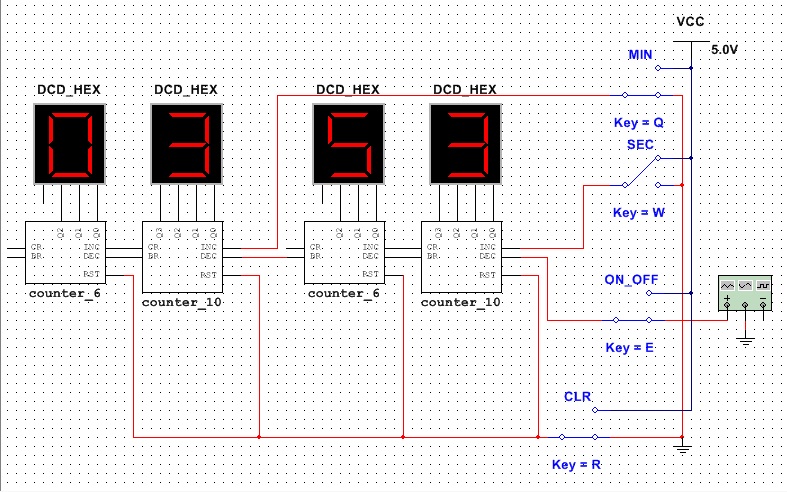
\includegraphics[width=\textwidth]{multisim/timer.png}
\caption[Uproszczony schemat timera.]{Uproszczony schemat timera w programie Multisim.}
\label{timer_scheme}
\end{figure}
\subsection{Implementacja w HDL.}
Poniżej przedstawiamy nadrzędny plik źródłowy projektu napisany w
języku Verilog. Występują w nim odniesienia do modułów, które
zostaną opisane w dalszej części sprawozdania. 
Pewne fragmenty zostały pominięte dla poprawy czytelności

\lstinputlisting[title=\texttt{UP2\textunderscore TOP.v}]{UP2_TOP_simp.v}
\section{Zegar 1Hz (\clocksec).}
\subsection{Opis układu.}
Do realizacji timera kluczowym elementem był \emph{zegar 1Hz},
umożliwiający dokładne odmierzenie jednej sekundy. 
W celu uzyskania z zegara 25,175MHz pożądanej częstotliwości, 
zastosowaliśmy preskaler.

Układ preskalera to 25-bitowy licznik modulo 25\,175\,000. 
Wyjście preskalera stanowi najstarszy, 24-ty bit jego rejestru. 
Rejestr jest zerowany, gdy licznik osiąga 25\,174\,999, co powoduje, że
częstotliwość sygnału wyjściowego wynosi 1Hz. Należy jednak
zaznaczyć, że wypełnienie zegara \emph{nie} jest równe 50\% .

\subsection{Implementacja w HDL.}
Z powodu zbyt dużego skomplikowania tego układu nie wykonaliśmy
symulacji w Multisimie. Poniżej zamieszczamy implementację zegara
1Hz w Verilogu.

\lstinputlisting[title=\clocksec .v]{clock_sec.v}
\section{Debouncer (\debouncer).}
\subsection{Opis układu.}
Podczas realizacji naszego projektu jednym z pierwszych problemów,
na jakie się natknęliśmy, były zakłócenia na stykach przycisków,
które występują w czasie naciskania. Dość szybko zdaliśmy sobie
sprawę, że potrzebujemy układu, który będzie te drgania eliminował,
znanego pod nazwą \emph{debouncer}.

Działanie debouncera polega na pomiarze czasu w jakim przycisk 
znajduje się w podanym stanie i rejestrowaniu przełączenia tylko 
gdy czas ten osiągnie pewną minimalną wartość. 
Minimalny czas $P$ potwierdzający stabilność zmiany wyraża wzór:
$$ 
P = \frac{2^N}{f} 
$$

Wartość P zależna jest od konstrukcji przycisku i może być wyznaczona
eksperymentalnie. Dla przycisków stosowanych w naszym projekcie przyjęliśmy
$P \approx 10\mathrm{ms}$.
$$
N = \lfloor\log_2(Pf)\rfloor
$$
Dla zegara 25,175MHz daje nam to $N=18$\ ($P=10,41$ms)
\subsection{Implementacja w HDL.}
Przełączniki stosowane przez nas w Multisimie na szczęście nie wymagają
debouncera. Poniżej przedstawiamy implementację w Verilogu.

\lstinputlisting[title=\debouncer .v]{debouncer.v}
\section{Liczniki (\counter{6}, \counter{10}).}
\subsection{Opis układu.}
\emph{Liczniki} to serce naszego układu. Odliczają w dół lub w
górę, w zależności od trybu, w którym znajduje się timer. Mogą też
zostać wyzerowane asynchronicznie wejściem \texttt{CLR}. Liczniki
są połączone ze sobą tak, aby po nastąpieniu \emph{przepełnienia}
--- wzrósł, zaś w przypadku \emph{niedomiaru} --- zmalał stan
licznika odpowiadającego za starszą cyfrę.

\counter{6} to licznik modulo 6, zaś \counter{10} --- modulo 10.
\subsection{Symulacja w Multisimie.}
Licznik modulo 6 to układ \emph{sekwencyjny} zbudowany na trzech
przerzutnikach. Sygnał podawany na wejście każdego przerzutnika jest
\emph{dekodowany} na podstawie aktualnego stanu wyjść licznika. Schemat pokazany jest na rysunku \ref{counter6_scheme}.
\begin{figure}[p]
\centering
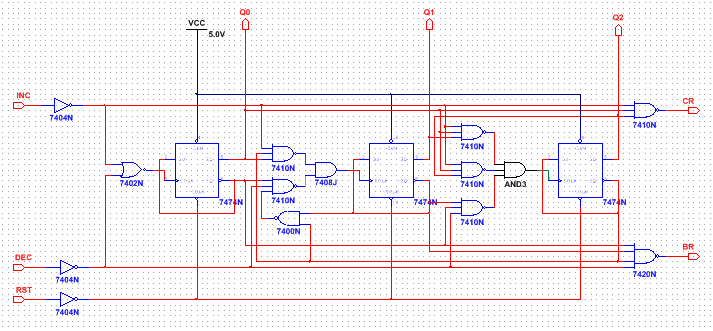
\includegraphics[width=\textwidth]{multisim/counter6.png}
\caption[Schemat licznika modulo 6.]{Schemat licznika modulo 6 w programie Multisim.}
\label{counter6_scheme}
\end{figure}

Licznik modulo 10 jest zbudowany podobnie. Główną różnicą jest tutaj
zastosowanie czterech przerzutników, co pozwala na zapamiętanie
wszystkich cyfr systemu dziesiętnego. Schemat na rysunku
\ref{counter10_scheme}.
\begin{figure}[p]
\centering
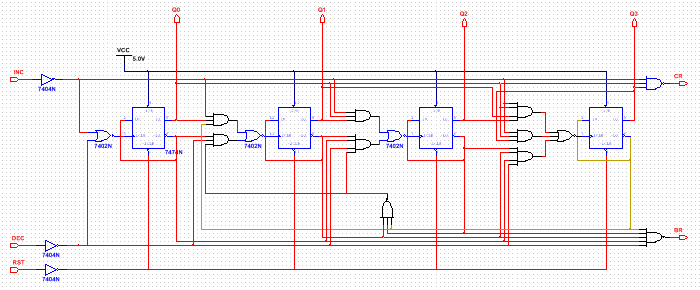
\includegraphics[width=\textwidth]{multisim/counter10.png}
\caption[Schemat licznika modulo 10.]{Schemat licznika modulo 10 w programie Multisim.}
\label{counter10_scheme}
\end{figure}
\subsection{Implementacja w HDL.}
Implementacja liczników w Verilogu to wyrażenie wcześniej
przedstawionych schematów w języku opisu sprzętu.

\lstinputlisting[title=\counter{6}.v]{counter_6.v}
\lstinputlisting[title=\counter{10}.v]{counter_10.v}
\section{Kontrola trybów (\mode).}
\subsection{Opis układu.}
Podczas projektowania układu ustaliliśmy, że timer będzie się mógł
znajdować w jednym z trzech \emph{trybów}: \texttt{RUN},
\texttt{HALT} i \texttt{BLINK} (wyjaśnienie poniżej). Dwa pierwsze
tryby mają większe znaczenie dla użytkownika i zostały opisane w
instrukcji, zaś trzeci z nich został wprowadzony po to, by
umożliwić sygnalizację zakończenia zliczania (miganie cyfr
na wyświetlaczu LED).

Z bardzo prostych obliczeń wynika, że chcąc zapamiętać 3 stany
potrzebujemy dwóch przerzutników. Nazwaliśmy je: \texttt{running} i
\texttt{ended}. Poniżej przedstawiony jest krótki opis znaczenia
każdego stanu wraz z przypisaną do niego 2-bitową wartością
rejestru \{\texttt{running}, \texttt{ended}\}:
\begin{enumerate}
\item \texttt{RUN} \{1,0\} --- tryb \emph{zliczania} --- liczniki
zliczają czas w dół, działanie wszystkich przycisków poza
\startstop\ jest zablokowane,
\item \texttt{HALT} \{0,0\} --- tryb \emph{ustawiania} --- liczniki
są zatrzymane, w tym trybie można dodawać minuty i sekundy, a także
resetować stan liczników,
\item \texttt{BLINK} \{0,1\} --- tryb \emph{migania} --- liczniki
są zatrzymane, działanie wszystkich przycisków poza \startstop\
jest zablokowane, a kropki na wyświetlaczu LED migają sygnalizując
koniec zliczania.
\end{enumerate}

Rysunek \ref{state_diagram} prezentuje przejścia pomiędzy trybami.
\begin{figure}[htbp]
\centering
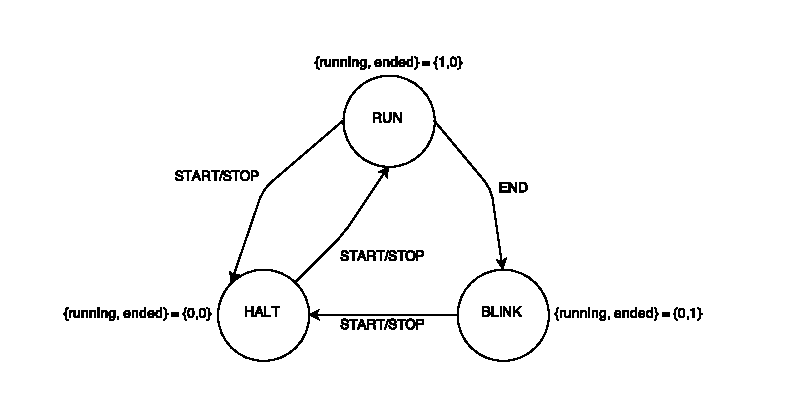
\includegraphics{state_diagram.pdf}
\caption[Diagram przejść pomiędzy trybami timera.]{Diagram przejść
pomiędzy trybami timera. \startstop\ oznacza zdarzenie naciśnięcia
przycisku \startstop , \texttt{END} oznacza zdarzenie zakończenia
zliczania.}
\label{state_diagram}
\end{figure}
\subsection{Implementacja w HDL.}
Zaimplementowaliśmy powyższy schemat w Verilogu. Sygnały
\startstop\ oraz \texttt{END} doprowadzone są do układu
odpowiednio poprzez wejścia: \texttt{btn} i
\texttt{end\textunderscore}. Na wyjście podawany jest stan
przerzutników \texttt{running} i \texttt{ended}.

\lstinputlisting[title=\texttt{mode.v}]{mode.v}
\section{Dekoder BCD na wyświetlacz 7-segmentowy (\bcdtoseg).}
\subsection{Opis układu.}
Aby użytkownik mógł widzieć stan timera na wyświetlaczu LED,
niezbędne jest \emph{zdekodowanie} sygnału pochodzącego od
liczników, w których cyfry pamiętane są w formacie BCD (Binary
Coded Decimal), na odpowiednie wejścia wyświetlacza 7-segmentowego.
W tym celu zbudowaliśmy układ, który nazwaliśmy \emph{Dekoderem
BCD na wyświetlacz 7-segmentowy}.

Dekoder jest układem \emph{kombinacyjnym}. To oznacza, że sygnał na
wyjściu zależy tylko i wyłącznie od sygnału na wejściu, w
odróżnieniu od układów \emph{sekwencyjnych}. Stan każdego wyjścia
jest opisany funkcją bool'owską, które realizowane są za pomocą
bramek logicznych.

\begin{table}[htbp] \caption{Tabela stanów logicznych} \label{decoder-table} \centering
\begin{tabular}{|c|cccc|ccccccc|} 
\hline 
& \multicolumn{4}{c|}{BCD} & \multicolumn{7}{c|}{7 segmentowy} \\
N  & Q3   & Q2   & Q1   & Q0  & G   & F  & E  & D  & C  & B  & A  \\ \hline
0  & 0    & 0    & 0    & 0   & 0   & 1  & 1  & 1  & 1  & 1  & 1  \\
1  & 0    & 0    & 0    & 1   & 0   & 0  & 0  & 0  & 1  & 1  & 0  \\
2  & 0    & 0    & 1    & 0   & 1   & 0  & 1  & 1  & 0  & 1  & 1  \\
3  & 0    & 0    & 1    & 1   & 1   & 0  & 0  & 1  & 1  & 1  & 1  \\
4  & 0    & 1    & 0    & 0   & 1   & 1  & 0  & 0  & 1  & 1  & 0  \\
5  & 0    & 1    & 0    & 1   & 1   & 1  & 0  & 1  & 1  & 0  & 1  \\
6  & 0    & 1    & 1    & 0   & 1   & 1  & 1  & 1  & 1  & 0  & 1  \\
7  & 0    & 1    & 1    & 1   & 0   & 0  & 0  & 0  & 1  & 1  & 1  \\
8  & 1    & 0    & 0    & 0   & 1   & 1  & 1  & 1  & 1  & 1  & 1  \\
9  & 1    & 0    & 0    & 1   & 1   & 1  & 0  & 1  & 1  & 1  & 1  \\
10 & 1    & 0    & 1    & 0   & x   & x  & x  & x  & x  & x  & x  \\
11 & 1    & 0    & 1    & 1   & x   & x  & x  & x  & x  & x  & x  \\
12 & 1    & 1    & 0    & 0   & x   & x  & x  & x  & x  & x  & x  \\
13 & 1    & 1    & 0    & 1   & x   & x  & x  & x  & x  & x  & x  \\
14 & 1    & 1    & 1    & 0   & x   & x  & x  & x  & x  & x  & x  \\
15 & 1    & 1    & 1    & 1   & x   & x  & x  & x  & x  & x  & x  \\ \hline
\end{tabular}
\end{table}

\begin{figure}[p] \caption{Tabele Karnaugh dla poszczególnych wyjść dekodera BCD na wyświetlacz 7-segmentowy.} \centering
\begin{Karnaugh}
\path (name) node {G}; \contingut{0,0,1,1,1,1,1,0,1,1,x,x,x,x,x,x}
\grp{12}{10}{orange}
\grp{2}{10}{green}
\grph{3}{10}{blue}
\grp[3pt]{4}{13}{red}
\end{Karnaugh}
%
\begin{Karnaugh}
\path (name) node {F}; \contingut{1,0,0,0,1,1,1,0,1,1,x,x,x,x,x,x}
\grp{0}{8}{green}
\grp{12}{10}{orange}
\grpv{4}{14}{blue}
\grp[3pt]{4}{13}{red}
\end{Karnaugh}

\begin{Karnaugh}
\path (name) node {E}; \contingut{1,0,1,0,0,0,1,0,1,0,x,x,x,x,x,x}
\grp{1}{11}{orange}
\grp{4}{13}{green}
\end{Karnaugh}
%
\begin{Karnaugh}
\path (name) node {D}; \contingut{1,0,1,1,0,1,1,0,1,1,x,x,x,x,x,x}
\grpone{4}{orange}
\grpone{1}{green}
\grpone{7}{blue}
\end{Karnaugh}

\begin{Karnaugh}
\path (name) node {C}; \contingut{1,1,0,1,1,1,1,1,1,1,x,x,x,x,x,x}
\grpone{2}{orange}
\end{Karnaugh}
%    
\begin{Karnaugh}
\path (name) node {B}; \contingut{1,1,1,1,1,0,0,1,1,1,x,x,x,x,x,x}
\grph{0}{10}{orange}
\grp{0}{8}{green}
\grp{3}{11}{blue}
\end{Karnaugh}

\begin{Karnaugh}
\path (name) node {A}; \contingut{1,0,1,1,0,1,1,1,1,1,x,x,x,x,x,x}
\grpone{4}{orange}
\grpone{1}{green}
\end{Karnaugh}    
\end{figure}

Dla każdego wyjścia sporządzamy osobną tabelę Karnaugh i na ich podstawie tworzymy funkcje logiczne:
\begin{align*}
A &= (Q_3 + \n{Q_2} + Q_1 + Q_0)(Q_3 + Q_2 + Q_1 + \n{Q_0}) &
  A &= Q_3 + Q_1 + \n{Q_2 \oplus Q_0} \\
B &= \n{Q_2} + Q_1Q_0 + \n{Q_1}\n{Q_0} &
  B &= \n{Q_2 (Q_1 \oplus Q_0)} \\
C &= Q_3 + Q_2 + \n{Q_1} + Q_0 &
  C &= Q_3 + Q_2 + \n{Q_1} + Q_0 \\
D &= A(Q_3 + \n{Q_2} + \n{Q_1} + \n{Q_0}) &
  D &= A(Q_3 + \n{Q_2 Q_1 Q_0})\\
E &= (\n{Q_0})(Q_1+\n{Q_2}) &
  E &= \n{Q_0 + \n{Q_1}Q_2 } \\
F &= Q_3 + Q_2\n{Q_1} + Q_2\n{Q_0} + \n{Q_1}\cdot\n{Q_0} &
  F &= Q_3 + \n{Q_1+Q_0} + Q_2\cdot\n{Q_1Q_0} \\
G &= Q_3 + \n{Q_0}Q_1 + Q_1\n{Q_2} + \n{Q_1}Q_2 &
  G &= Q_3 + \n{Q_0}Q_1 + (Q_1 \oplus Q_2)   \\
\end{align*}

\subsection{Symulacja w Multisimie.}
Na rysunku \ref{decoder_scheme} przedstawiamy implementację
uzyskanych funkcji na bramkach logicznych w programie Multisim.
\begin{figure}[p]
\centering
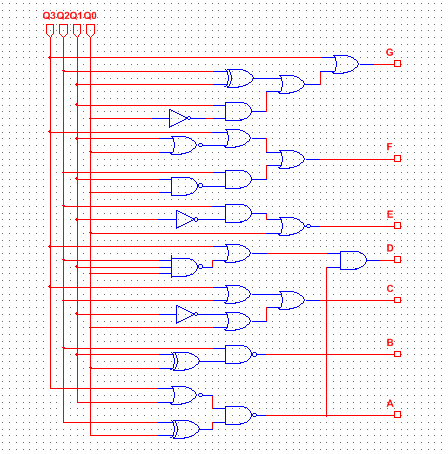
\includegraphics[width=\textwidth]{multisim/bcdto7seg.png}
\caption[Schemat dekodera BCD na wyświetlacz 7-segmentowy.]{Schemat dekodera BCD na wyświetlacz 7-segmentowy w programie Multisim.}
\label{decoder_scheme}
\end{figure}
\subsection{Implementacja w HDL.}
Aby zaimplementować dekoder w Verilogu wystarczy podać, jakiego
zestawu stanów na wyjściu oczekujemy dla każdego zestawu stanów na
wejściu. Kompilator automatycznie będzie się starał zoptymalizować
układ bramek logicznych realizujący podaną w ten sposób
\emph{tabelę prawdy}.

\lstinputlisting[title=\bcdtoseg .v]{bcd_to_7seg.v}

\end{document}
